%-----------------------------------------
% Resume Template in English
% Designed by Mitra Babaei
% Summer 2024
%-----------------------------------------
\documentclass[oneside]{article}

\usepackage{wallpaper}
\usepackage{geometry}
\usepackage[
    unicode=true,
    bookmarks=true,
    bookmarksnumbered=false,
    bookmarksopen=true,
    bookmarksopenlevel=1,
    breaklinks=false,
    pdfborder={0 0 0},
    backref=false,
    colorlinks=false
    ]{hyperref}
\usepackage{lastpage}
\usepackage{hyphenat}
\usepackage{hyphsubst}
\usepackage{tabularx}
\usepackage{moresize}
\usepackage[document]{ragged2e}
\usepackage[scaled]{helvet}
\usepackage{fontawesome5}
\usepackage[defaultfam,tabular,oldstyle]{montserrat}
\usepackage[T1]{fontenc}
\usepackage{titlesec}
\usepackage{xcolor}
\usepackage{tikz}
\renewcommand*\oldstylenums[1]{{\fontfamily{Montserrat-TOsF}\selectfont #1}}
\setlength{\parindent}{0pt}
\titleformat{\section}{\normalfont}{}{0pt}{}
\renewcommand{\arraystretch}{1.4}
\setlength\fboxrule{0pt}
\setlength\fboxsep{10pt}
\titlespacing{\section}{0pt}{1.5ex plus .1ex minus .2ex}{1pc}
\newcolumntype{Y}{>{\RaggedRight\arraybackslash}X}

%-----------------------------------------
%
%     Change PDF Meta Info here
%
%-----------------------------------------

\hypersetup{
    pdftitle={Atefeh Aghababaei - CV - English},
    pdfauthor={Atefeh Aghababaei},
    pdfsubject={CV}
}

% Paper size
\geometry{
    a4paper,
    left=0pt,
    right=20pt,
    top=0pt,
    bottom=0pt,
    nohead,
    % includefoot,
    nomarginpar
}

% Background Color of the Sidebar Column
\definecolor{sidebg}{cmyk}{0.17, 0.14, 0.14, 0.02}

% Background Color of the Main Column
\definecolor{mainbg}{cmyk}{0, 0, 0, 0}

% Text Color of the Main Column
\definecolor{maintext}{cmyk}{1, 0.02, 0, 0.8}

% Text Color of the Sidebar Column
\definecolor{sidetext}{cmyk}{1, 0.02, 0, 0.8}

\pagecolor{mainbg}

%-----------------------------------------
\usepackage[most]{tcolorbox} % Load the tcolorbox package

\newtcbox{\cvtag}[1][]{%
  on line,
  arc=2pt, outer arc=2pt,
  colback=sidebg, % Use the custom color for the background
  opacityback=1, % Background opacity (1 for solid)
  colframe=lightgray!50!sidebg, % Frame color
  coltext=white, % HERE: Set the text color to white
  boxsep=0pt,
  left=1pt, right=1pt, top=2pt, bottom=2pt,
  box align=base,
  #1}
%-----------------------------------------

\begin{document}
\setlength{\topskip}{0pt}\setlength{\footskip}{0pt}%
\fcolorbox{red}{sidebg}{%
    \begin{minipage}[t][\textheight-2\fboxsep-2\fboxrule][t]{\dimexpr0.41\textwidth-2\fboxrule-2\fboxsep\relax}
    
        \color{sidetext}
        %-----------------------------------------
        % YOUR NAME, PRONOUNS, OCCUPATION(s), AND HEADSHOT
        %-----------------------------------------
        \begin{center}
            \begin{tikzpicture}
            \clip (0,0) circle (3.015cm) node[anchor=center] {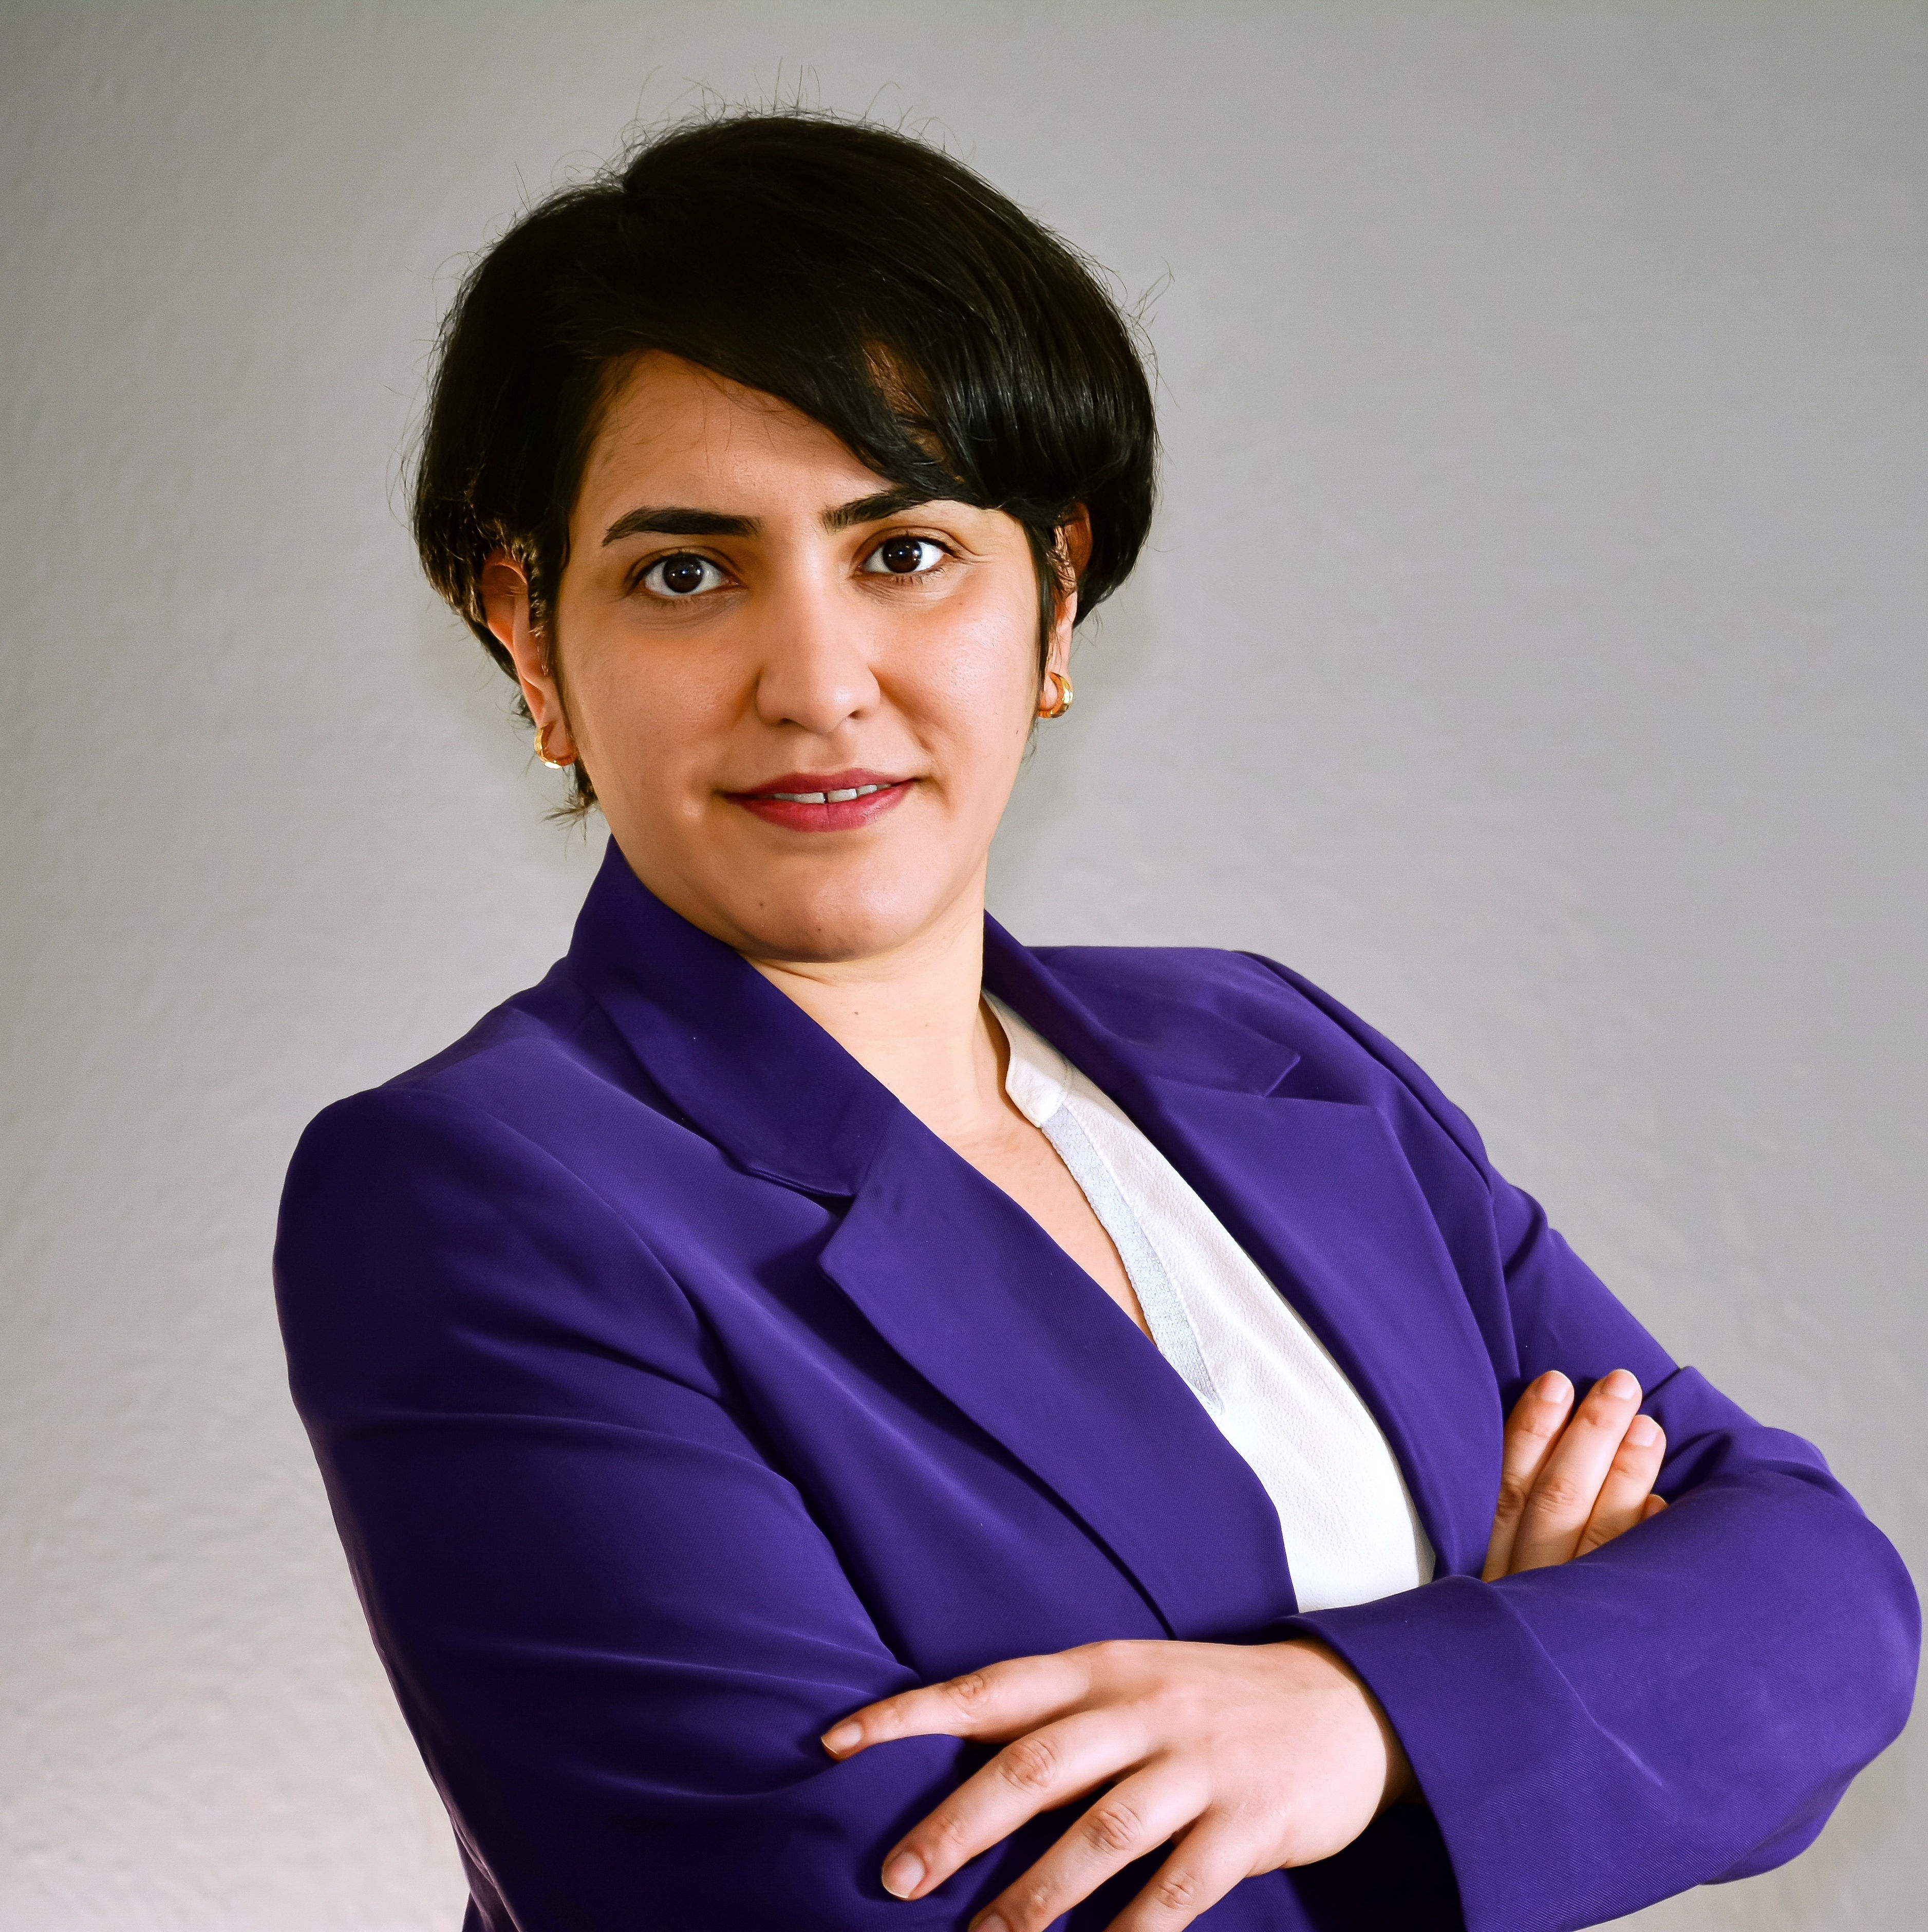
\includegraphics[width=6cm]{photos/business_foto.jpg}};
            \end{tikzpicture}
        \end{center}
        %\vspace{.3cm}
        {\bfseries Dr. rer. nat.} \\
        \vspace{.2cm}
        {\bfseries\huge Atefeh} \\
        \vspace{.2cm}
        {\bfseries\huge Aghababaei} %\qquad {they/them}
        \vspace{.2cm} \\
        Physicist | Data Scientist %| Imaging Specialist
        \vspace{7pt} \\
        %-----------------------------------------
        % YOUR LINKS, YOU MAY ALSO ADD A PERSONAL WEBSITE OR PORTFOLIO
        %-----------------------------------------
        \rule{\linewidth}{0.35pt} \\
        \phantomsection{}
        \addcontentsline{toc}{section}{Contact}
        \section*{\large Contact}
        \begin{tabularx}{\textwidth}{@{}lX@{}}%{cY}
            \faPhone{}      & +49 177 4922042 \\
            \faEnvelope{}   & \href{mailto:atefehbabaei90@gmail.com}{atefehbabaei90@gmail.com} \\
            \faMapMarker{}  & {Paul-Schall\"uck Str. 21, 50939 K\"oln} \\
            \faLinkedin{}   & \href{https://www.linkedin.com/in/atefeh-babaei/}{/atefeh-babaei} \\
            %\faXing{}       & \href{https://www.xing.com/profile/AtefehMitra_Aghababaei}{/AtefehMitra\_Aghababaei} \\
            %\faCode{}     & \href{https://example.com}{example.com} \\
            \faGithub{}   & \href{https://github.com/mitibabaei}{/mitibabaei} \\
        \end{tabularx}
        \vspace{1pt} \\
        \rule{\linewidth}{0.4pt} \\
        %-----------------------------------------
        % YOUR PERSONAL INFROMATION
        %-----------------------------------------
        \phantomsection{}
        \addcontentsline{toc}{section}{Personal info}
        \section*{\large Personal Info}
        \begin{tabularx}{\textwidth}{@{}lX@{}}
            %\faStarOfLife{} & Date of Birth: 17/05/1990 \\
            \faFlag{}       & Citizenships: German $\bullet$ Iranian \\
            
        \end{tabularx}
        \vspace{1pt} \\
        \rule{\linewidth}{0.4pt} \\
        %-----------------------------------------
        % YOUR SKILLS
        %-----------------------------------------
        \phantomsection{}
        \addcontentsline{toc}{section}{Skills}
        \section*{\large Skills}
        
        \begin{tabularx}{\textwidth}{@{}lX@{}} % Adjusted for no extra space at start and end of table
            \faLanguage{}   & \textbf{\footnotesize Languages} \newline English  $\bullet$  German (B2) $\bullet$ Persian \\
            
            \faCode{}        & \textbf{\footnotesize Programming} \newline Python $\bullet$ Bash $\bullet$ SQL $\bullet$  R $\bullet$ MATLAB. \\
            
            \faLaptopCode{}  & \textbf{\footnotesize Data Science \& Analysis Tools} \newline Pandas $\bullet$ Matplotlib $\bullet$  NumPy $\bullet$ SciPy $\bullet$ Scikit-learn $\bullet$ PyTorch $\bullet$ Jupyter. \\
            
            \faCogs{}        & \textbf{\footnotesize Technical Skills} \newline Data Visualization $\bullet$ Data Analytics$\bullet$ Image Processing $\bullet$ Machine Learning $\bullet$ Data Mining $\bullet$ Data management $\bullet$ Big Data $\bullet$ Statistics Methods. \\ %  $\bullet$ Statistics MethodsTroubleshooting
            
            \faToolbox{}     & \textbf{\footnotesize Project Management} \newline Agile Methodologies $\bullet$ Scrum $\bullet$ Project Planning $\bullet$ Confluence $\bullet$ Jira. \\
            
            \faCloud{}       & \textbf{\footnotesize Cloud Computing}  \newline Fundamentals of Cloud Computing.% $\bullet$ Google Cloud. 
            \\
        
            \faUsers{}       & \textbf{\footnotesize Soft Skills} \newline Strategic Management $\bullet$ Team Work $\bullet$ Presentation $\bullet$ Decision Making $\bullet$ Critical Thinking $\bullet$ Problem Solving. \\
        \end{tabularx}

        \vspace{1pt}
        
    \end{minipage}
}
\hfill
\fcolorbox{red}{mainbg}{%
    \begin{minipage}[t][\dimexpr\textheight-2\fboxrule-2\fboxsep\relax][t]{\dimexpr0.6\textwidth-2\fboxrule-2\fboxsep\relax}
        \color{maintext}
        \vspace{17pt}
        %-----------------------------------------
        % brief introduction or summary of your professional background, skills, and career goals.
        %-----------------------------------------
        {\footnotesize \justify Data scientist with PhD in Physics and over six years of experience in developing Python tools to process and analyze large datasets.
        My work also extends to image processing and visualization, where I have applied advanced techniques to derive actionable insights.
        My strength is in tackling complex questions by creating or adapting agile approaches, as well as leading projects with a focus on fostering a collaborative spirit within the team.}
        %-----------------------------------------
        % WORK EXPERIENCE
        %-----------------------------------------
        \phantomsection{}
        \addcontentsline{toc}{section}{Work Experience}
        \section*{\scshape\Large Work Experience \rule{\linewidth}{0.4pt}}
        
        {\large \textbf{Researcher / Data Scientist}} \\ 
        {\scshape\fontseries{light}\selectfont\footnotesize University of Cologne \qquad May 2017 \textendash{} Sep. 2023} \\

        \begin{itemize}
            \setlength{\itemsep}{-3pt}
            \footnotesize
            %\item Analyzed complex observations of the massive star formation region NGC6334-V.
            \item Developed Python pipelines for image processing techniques, big data analysis, and visualization.
            \item Led peer-reviewed scientific articles and published in renowned journals.
            \item Collaborated with external scientists and established global connections. 
            \item Presented results in both talks and poster formats at tens of international workshops and conferences.
            \item Trained, and supervised Master and bachelor\textendash{}level students.
            \item Teacher assistant for four Master and bachelor\textendash{}level lectures.
            \item Member of the Collaborative Research Centers (CRC\textendash{}956) funded by DFG.
            
        \end{itemize}
%
        {\large \textbf{Research Assistant}} \\
        {\scshape\fontseries{light}\selectfont\footnotesize Max Planck Institute for Radio Astronomy (MPIFR) \qquad May 2014 \textendash{} May. 2016} \\
        
        \begin{itemize}
            \setlength{\itemsep}{-3pt}
            \footnotesize
            \item Evaluated phasing of ALMA telescopes regression test data sets.
            \item Calibrated and visualized telescope sample data sets.
            \item Compared calibration methods for various radio telescope data sets.
            \item Managed the reception, storage, and transfer of observational data at the VLBI Data Center.
        \end{itemize}
        
        %-----------------------------------------
        % EDUCATION
        %-----------------------------------------
        \phantomsection{}
        \addcontentsline{toc}{section}{Education}
        \section*{\scshape\Large Education \rule{\linewidth}{0.4pt}}
%
        {\large \textbf{Ph.D. \textendash{} Physics }} \\
        {\scshape\fontseries{light}\selectfont\footnotesize University of Cologne \qquad Feb 2019 \textendash{} Oct. 2023} \\
        {\footnotesize Title: Dr. rer. nat.} \\%[1ex]
        {\footnotesize Subject: Experimental Physics / Astrophysics} \\
        {\footnotesize Dissertation Title: Kinematics and Structure of Massive Star Formation in NGC6334-V} \\[2ex]

        {\large \textbf{M.Sc. \textendash{} Physics}} \\
        {\scshape\fontseries{light}\selectfont\footnotesize Bonn\textendash{}Cologne Graduate School \qquad Apr 2016 \textendash{} Aug. 2018} \\
        {\footnotesize Subject: Experimental Physics / Astrophysics} \\
        {\footnotesize Dissertation Title: Characterizing the High Mass Protocluster NGC6334-V via High-Resolution ALMA Observations} \\
        %-----------------------------------------
        % Certifications
        %-----------------------------------------
        \phantomsection{}
        \addcontentsline{toc}{section}{Certifications}
        \section*{\scshape\Large Certifications \rule{\linewidth}{0.4pt}}
        \noindent
        {\footnotesize \textbf{SQL}} \newline { \footnotesize SQLite Essential Training}\\
        {\footnotesize \textbf{Project Management Foundations}} \newline { \footnotesize Ethics $\bullet$ Requirements $\bullet$ Schedules $\bullet$ Budgets $\bullet$ Teams $\bullet$ Communications $\bullet$ Risk $\bullet$ Stakeholders}\\
        {\footnotesize \textbf{Cloud Concepts}} \newline { \footnotesize Cloud Architecture $\bullet$ Cloud Computing $\bullet$ Cloud Security $\bullet$ Determining Cloud Strategy $\bullet$ IBM Certified Cloud Professional Architect}
    
        %-----------------------------------------
        % Voluntary Activities
        %-----------------------------------------
        \phantomsection{}
        \addcontentsline{toc}{section}{Voluntary Activities}
        \section*{\scshape\Large Voluntary Activities \rule{\linewidth}{0.4pt}}
%
        \noindent

        {\footnotesize \textbf{First Speaker and Main Member} \footnotesize of CRC\textendash{}956 Students Council} \\
        {\scshape\fontseries{light}\selectfont\footnotesize University of Cologne \qquad Jun 2019 \textendash{} Nov. 2021} \\

        {\footnotesize \textbf{Organizing Committee} \footnotesize of the Assembly of the European Astronomical Society } \\
        {\scshape\fontseries{light}\selectfont\footnotesize Leiden (Virtual) \qquad Jun 2021 \textendash{} Jul. 2021} \\
        
        {\footnotesize \textbf{Organizing Committee} \footnotesize of the 30th General Assembly of the International Astronomical Union} \\
        {\scshape\fontseries{light}\selectfont\footnotesize Vienna \qquad Aug. 2018 } \\
        \vspace{20pt}

        %-----------------------------------------
        \noindent
        \begin{minipage}[c]{0.95\textwidth} 
        \flushright
        %\hfill
        \footnotesize K\"oln, \qquad \today \\
        \footnotesize Dr. Atefeh Aghababaei
        \end{minipage}%
        
    \end{minipage}
}%


\end{document}
